\documentclass{article}
\usepackage{graphicx}
\usepackage{afterpage}
\usepackage{setspace}

\begin{document}

\begin{titlepage}
    \centering
    \includegraphics[width=12cm]{images/20090516224137!Logotip_KBTU (1) (1).jpg}
    
    \vspace{0cm} % Add vertical space
    {\fontsize{40}{48}\selectfont Факультет Информационных систем} % Large font size and the text you mentioned
    
    \vspace{0.1cm} % Add vertical space
    
    \begin{center} % Center the following text
        Faculty of Information Technology\\
        Department of Electrical Engineering and Computer Science
    \end{center}
    
    \vfill % Fill the vertical space
    
    {\LARGE\bfseries Laboratory Work \#4}\\
    {\LARGE\bfseries Energy storage}
    {\LARGE\bfseries Elements}
    \vspace{4cm} % Add vertical space
    
    \begin{flushright}
        Done by: Sagingaly Meldeshuly \\
        Checked by: Raushan Amanzholova \\
        September 2023
    \end{flushright}
    
    \vfill % Center the page number vertically
    \begin{center}
        2023, Almaty
    \end{center}
    
\end{titlepage}



% "*" убирает нумерацию в разделе section
% "$ $" в долларах мы пишем математических операций
% " \times " это умножение с крестиком
% P_R_2=$I_R_2 \times V_R_2$
% \[ numerator and denominator
%\frac{a}{b}
%\]
% power ^
% \subsection подтопик
% Omega
% \\ is used to create a new line or break a line. It's similar to pressing "Enter" or "Return" on your keyboard when you're writing a regular text document.
\begin{flushleft}
\textbf{Purpose of the work laboratory work:}
\end{flushleft}
\begin{enumerate}
    \item Find all currents by KCL and KVL.
    \item Find all currents by Mesh analysis.
    \item Find all currents by Nodal analysis.
    \item Find all currents by Superposition.
\end{enumerate}

\begin{flushleft}
\textbf{Brief theory}
\end{flushleft}

\begin{flushleft}
The laboratory work focused on various methods for analyzing electrical circuits and determining currents, contributing to a comprehensive understanding of circuit analysis. Here is a brief theory explaining the methods used:

\begin{itemize}
    \item **Kirchhoff's Voltage Law (KVL) and Kirchhoff's Current Law (KCL):** KVL states that the algebraic sum of voltage drops in any closed loop of a circuit is zero, while KCL states that the total current entering a junction equals the total current leaving it. These laws are fundamental for analyzing complex circuits, as they provide a basis for current and voltage calculations.

    \item **Mesh Analysis:** Mesh analysis simplifies circuit analysis by dividing the circuit into individual loops or meshes. It relies on KVL to formulate equations for each mesh, making it particularly useful for circuits with numerous current sources.

    \item **Nodal Analysis:** Nodal analysis focuses on the voltage at circuit nodes. It uses KCL to establish equations for each node in the circuit, allowing for the calculation of various branch currents. Nodal analysis is effective when dealing with circuits that have voltage sources.

    \item **Superposition:** Superposition is a method that simplifies complex circuits by analyzing them one source at a time while considering all other sources as inactive. This technique is valuable for understanding how each source contributes to the overall circuit behavior and allows for more precise current calculations.
\end{itemize}
\end{flushleft}

\begin{flushleft}
\textbf{Pre lab tasks}
\end{flushleft}


\begin{flushleft}
    \begin{titlepage}
    \centering
    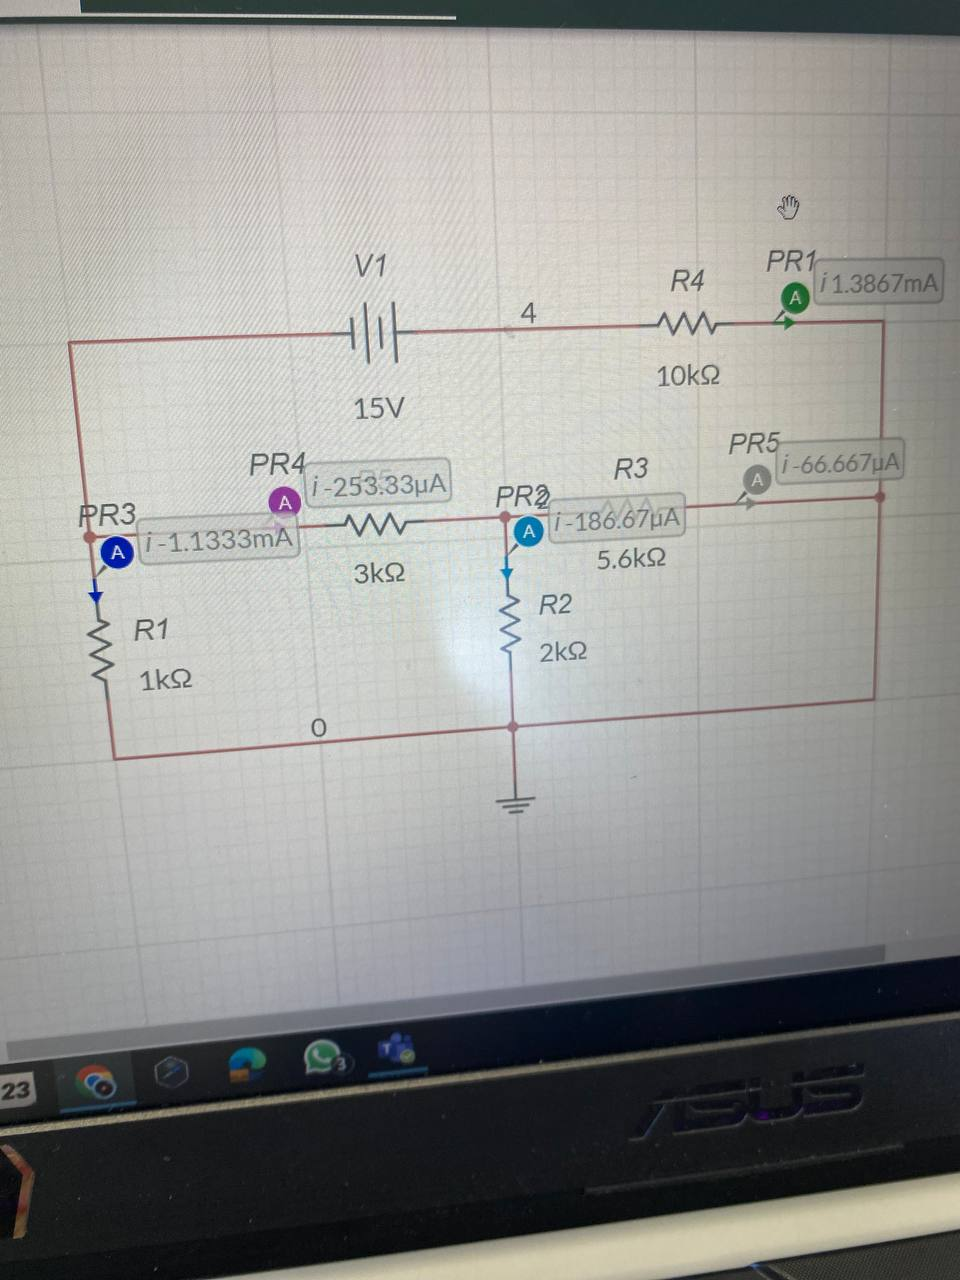
\includegraphics[width=14cm]{images/photo1696868902 (2).jpeg}
\end{flushleft}

\begin{flushleft}
    \centering
    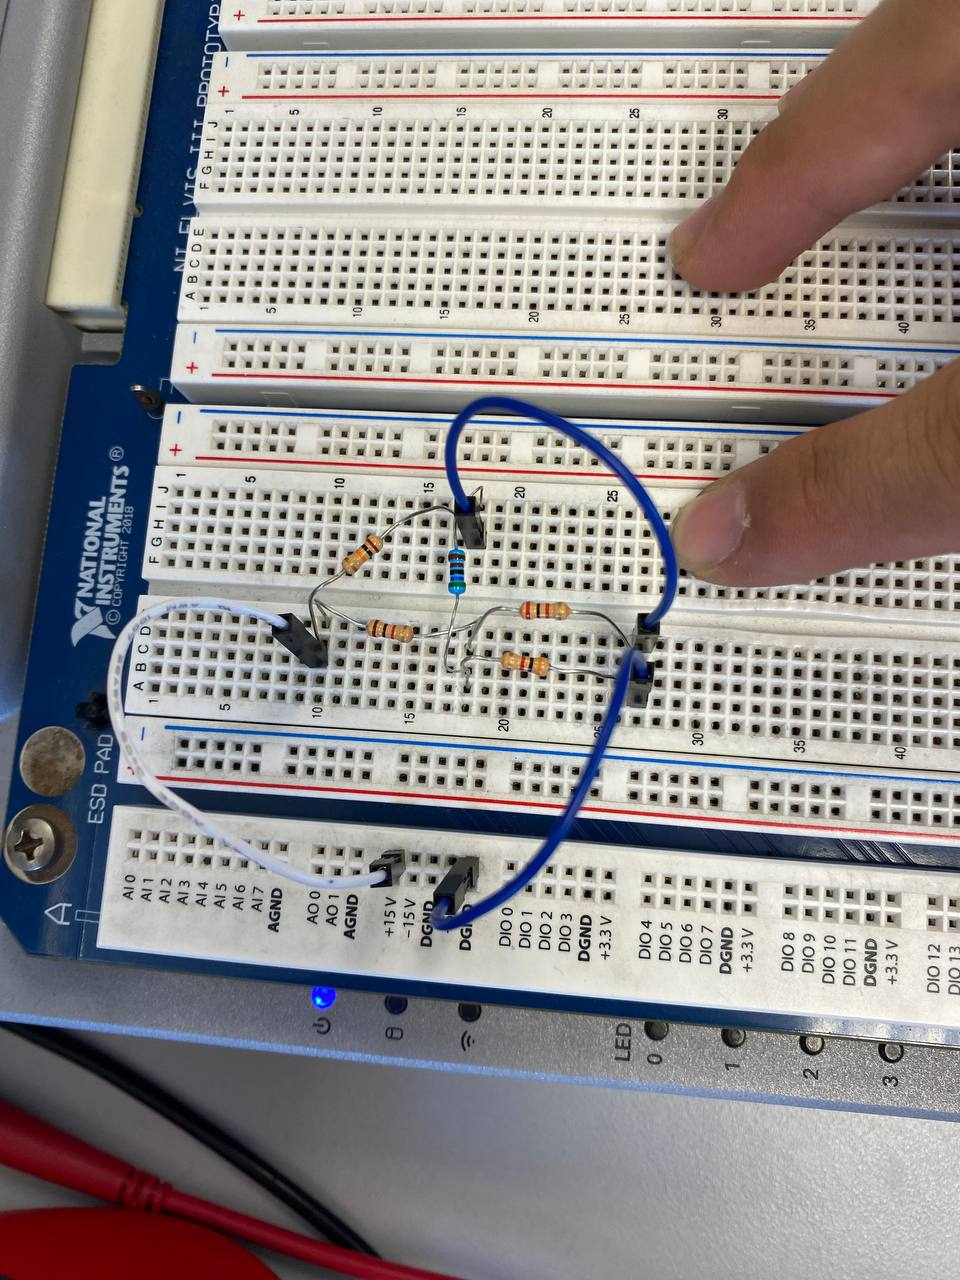
\includegraphics[width=14cm]{images/photo1696868715 (1).jpeg}
\end{flushleft}


\begin{flushleft}
    \begin{titlepage}
    \centering
    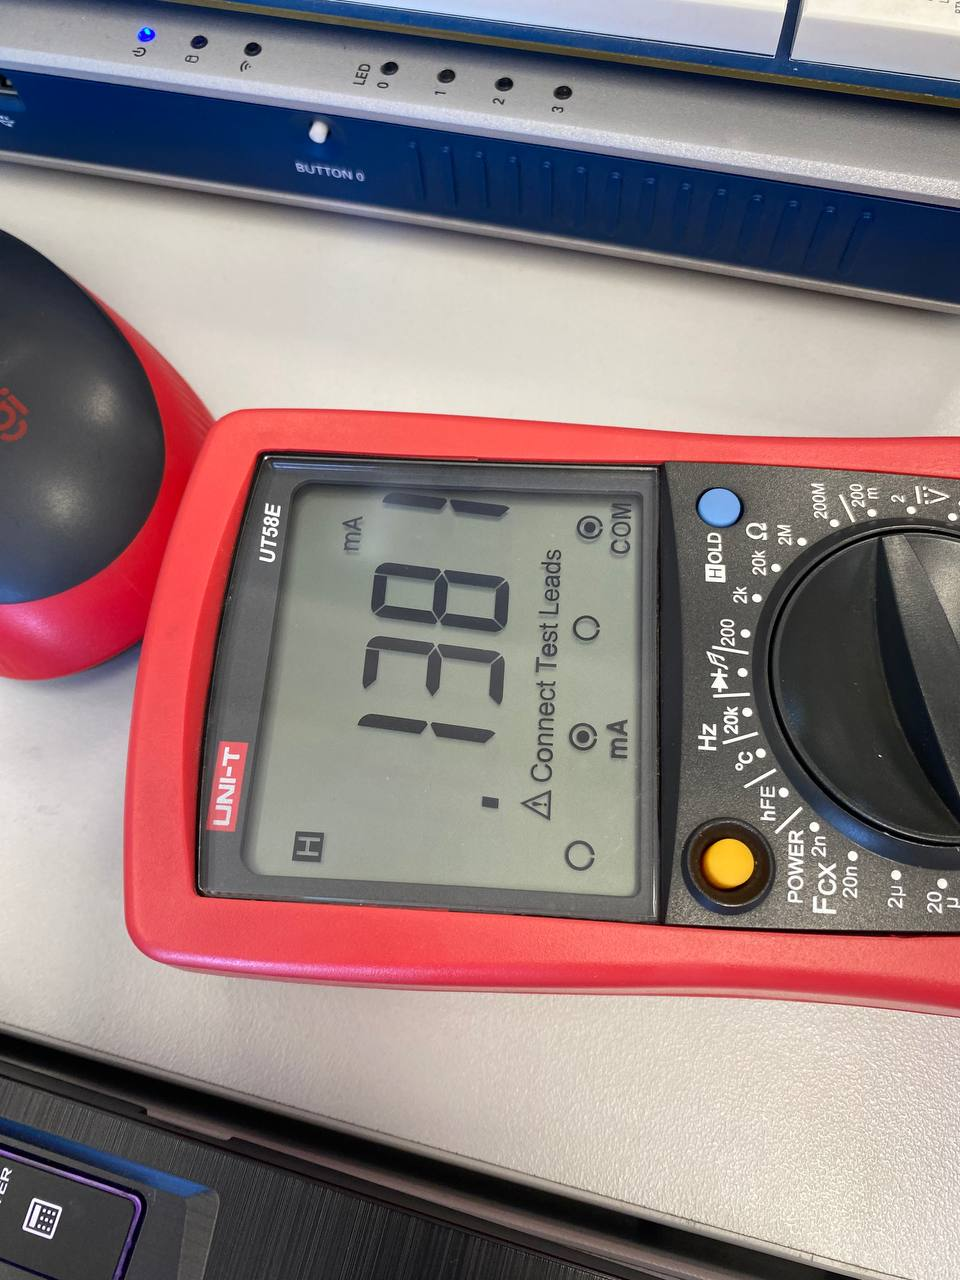
\includegraphics[width=14cm]{images/photo1696868715 (7).jpeg}
\end{flushleft}

\begin{flushleft}
    \begin{titlepage}
    \centering
    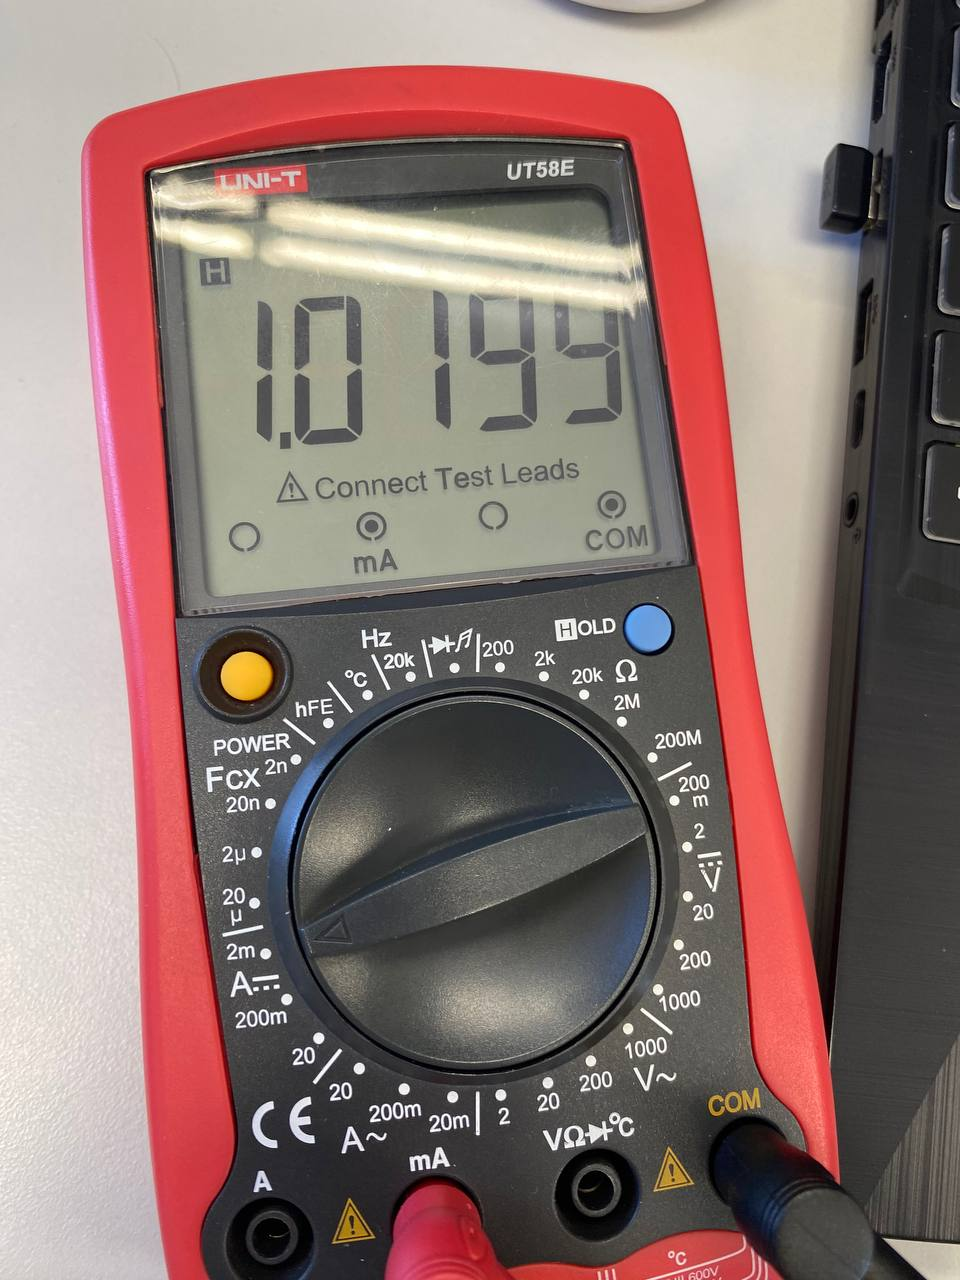
\includegraphics[width=14cm]{images/photo1696868715 (6).jpeg}
\end{flushleft}

\begin{flushleft}
    \centering
    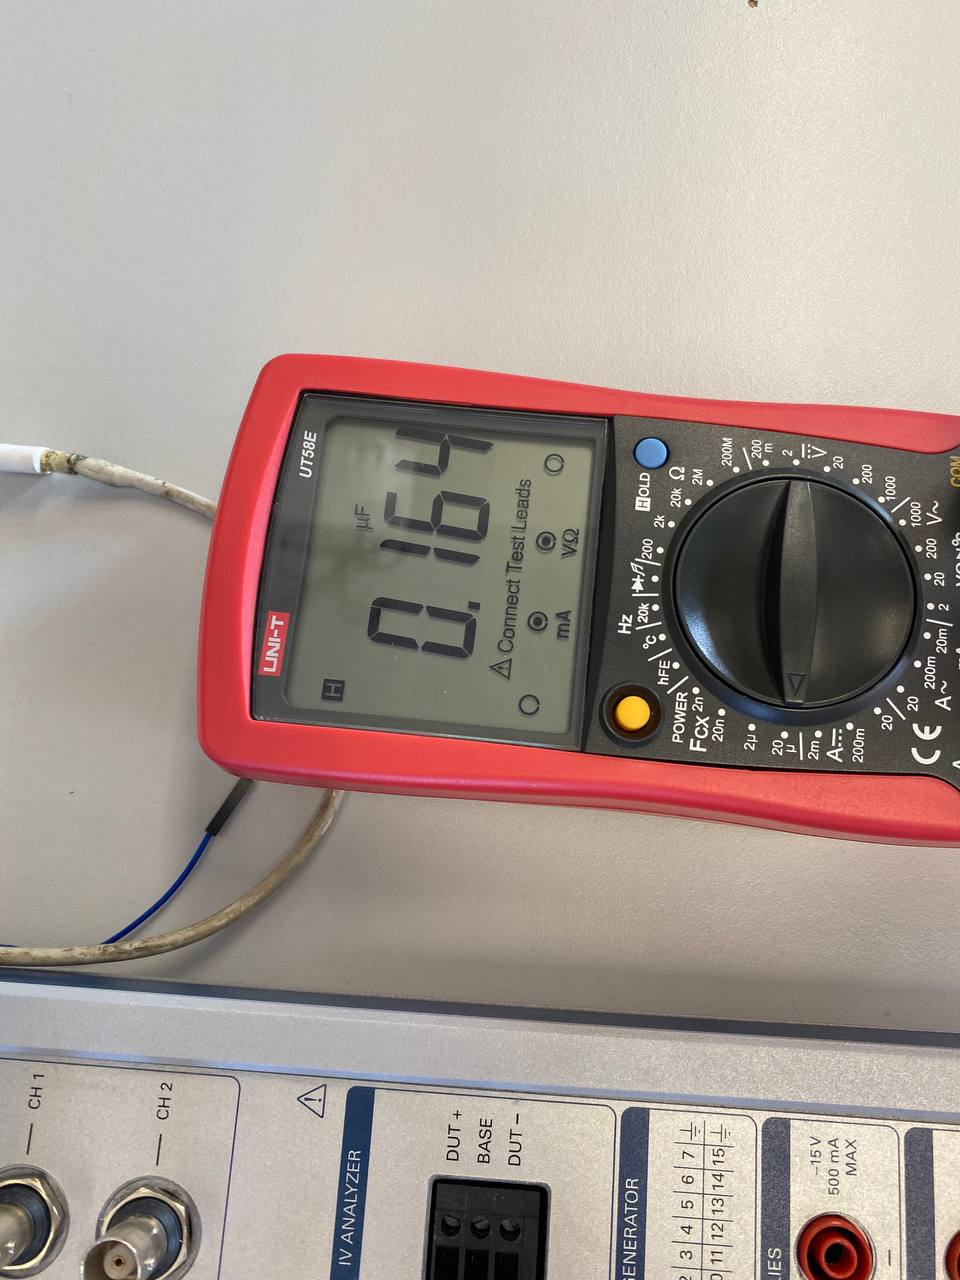
\includegraphics[width=14cm]{images/photo1696868715 (5).jpeg}
\end{flushleft}


\begin{flushleft}
    \centering
    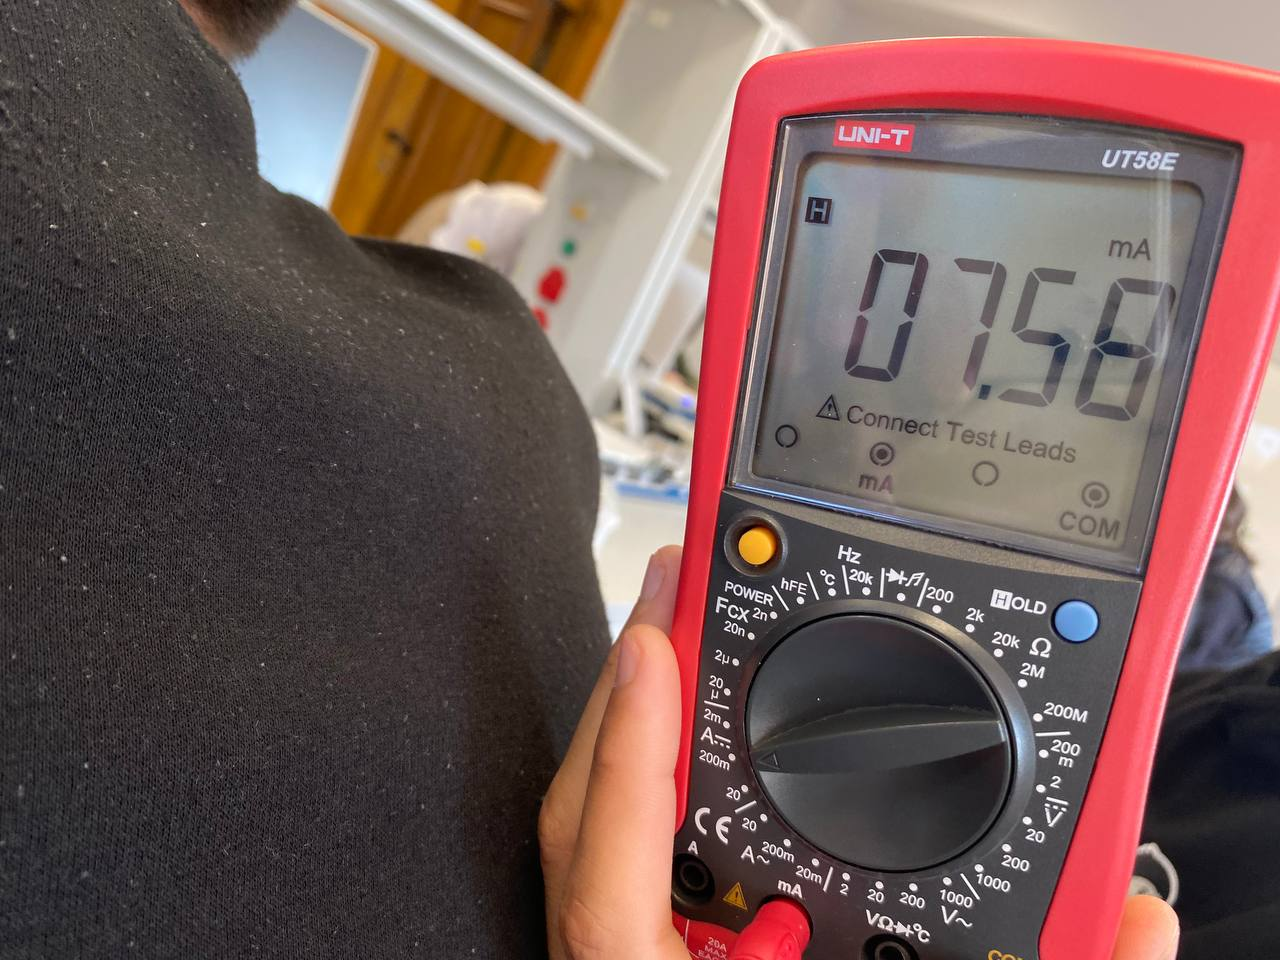
\includegraphics[width=14cm]{images/photo1696868715 (4).jpeg}
\end{flushleft}

\begin{flushleft}
    \centering
    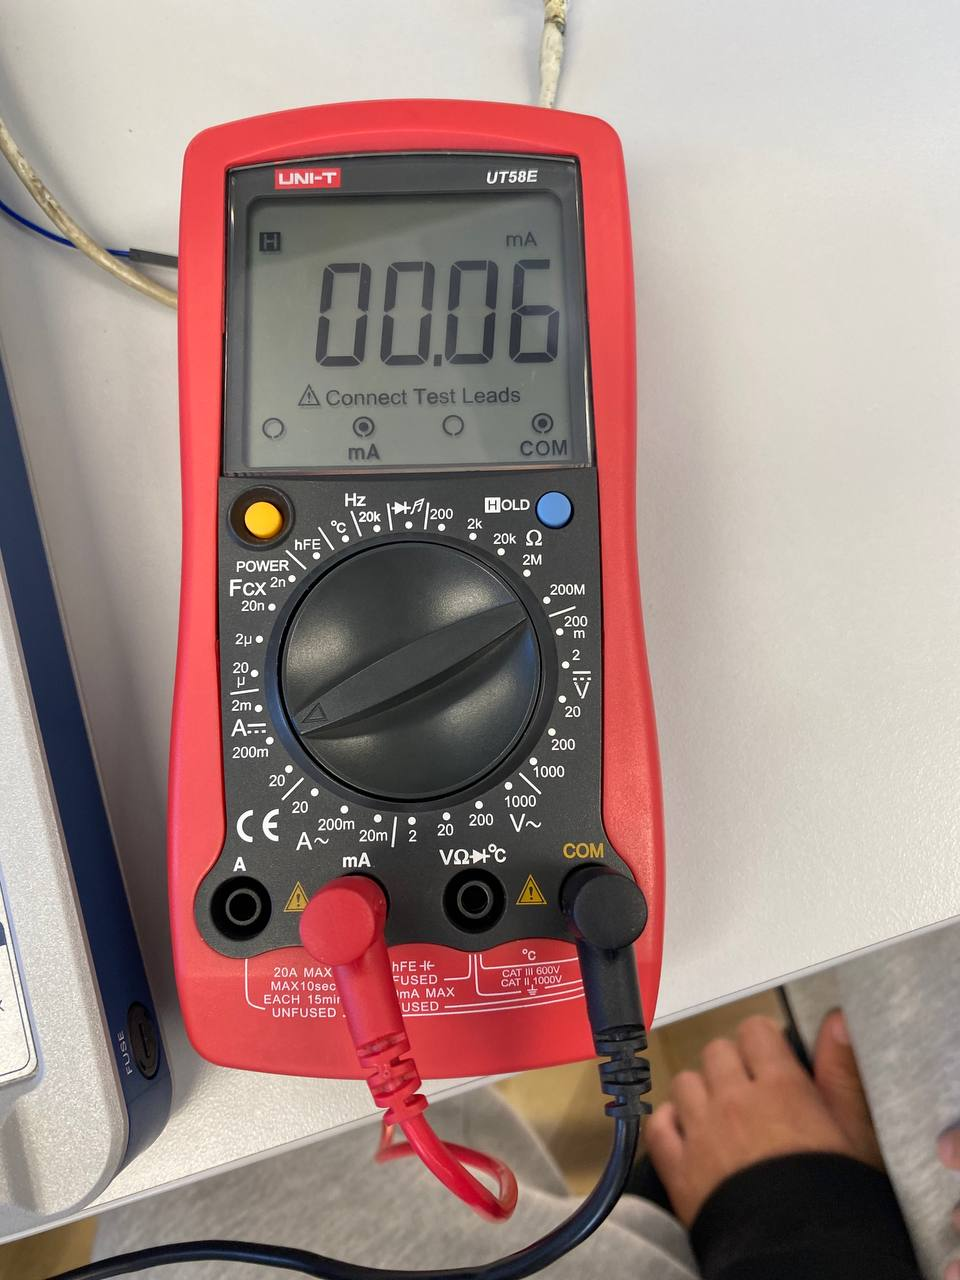
\includegraphics[width=15cm]{images/photo1696868715 (3).jpeg}
\end{flushleft}

\begin{flushleft}
\textbf{In lab tasks}
\end{flushleft}

Connect your circuit to Elvis Evaluation Board, and get measurements. Compare with in- lab results.

\begin{flushleft}
    \begin{titlepage}
    \centering
    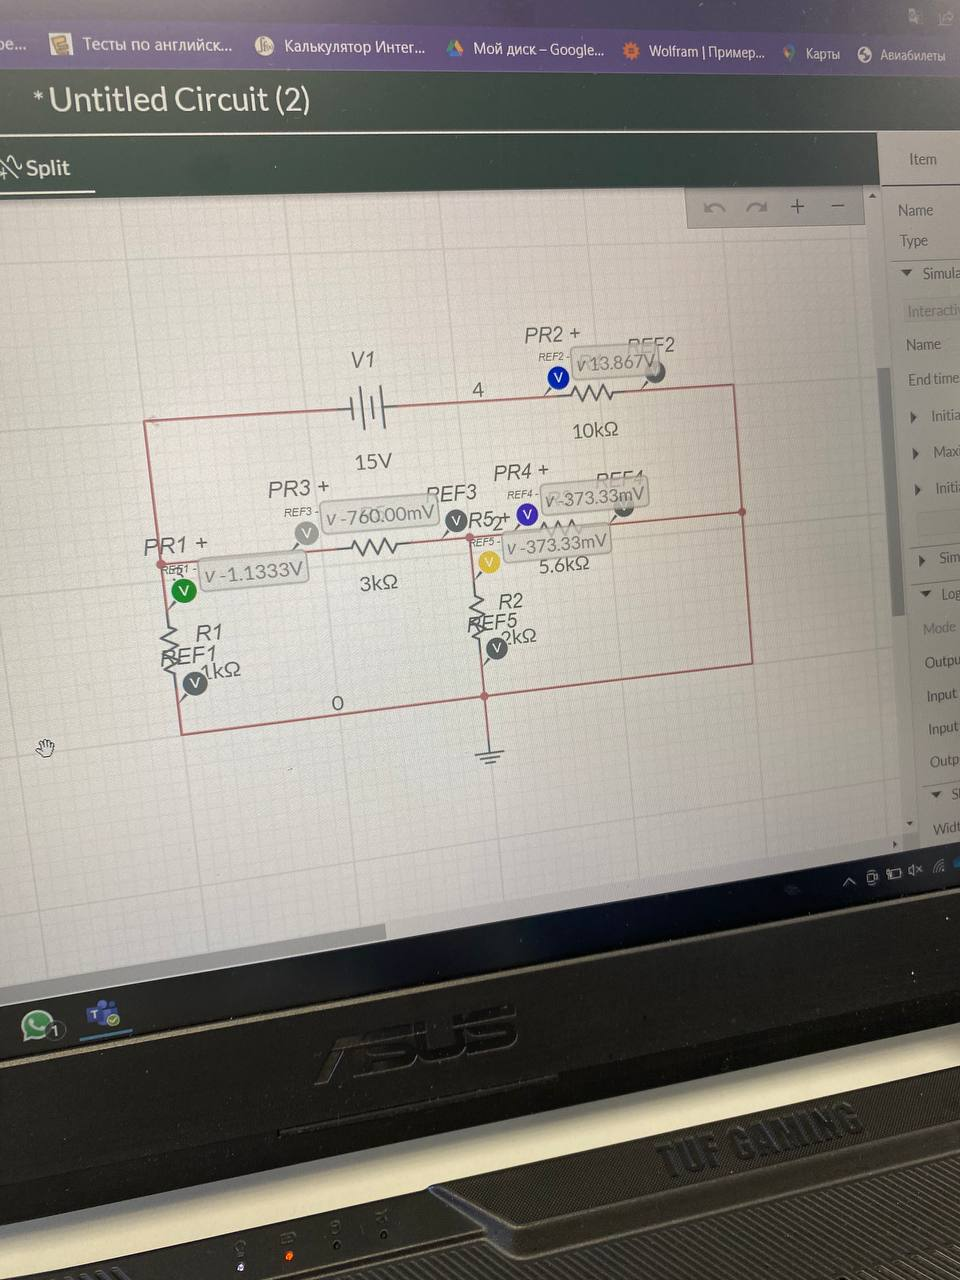
\includegraphics[width=14cm]{images/photo1696868715 (2).jpeg}
\end{flushleft}



\begin{flushleft}
    \begin{titlepage}
    \centering
    \includegraphics[width=14cm]{images/electric.jpeg}
\end{flushleft}

\begin{flushleft}
    \begin{titlepage}
    \centering
    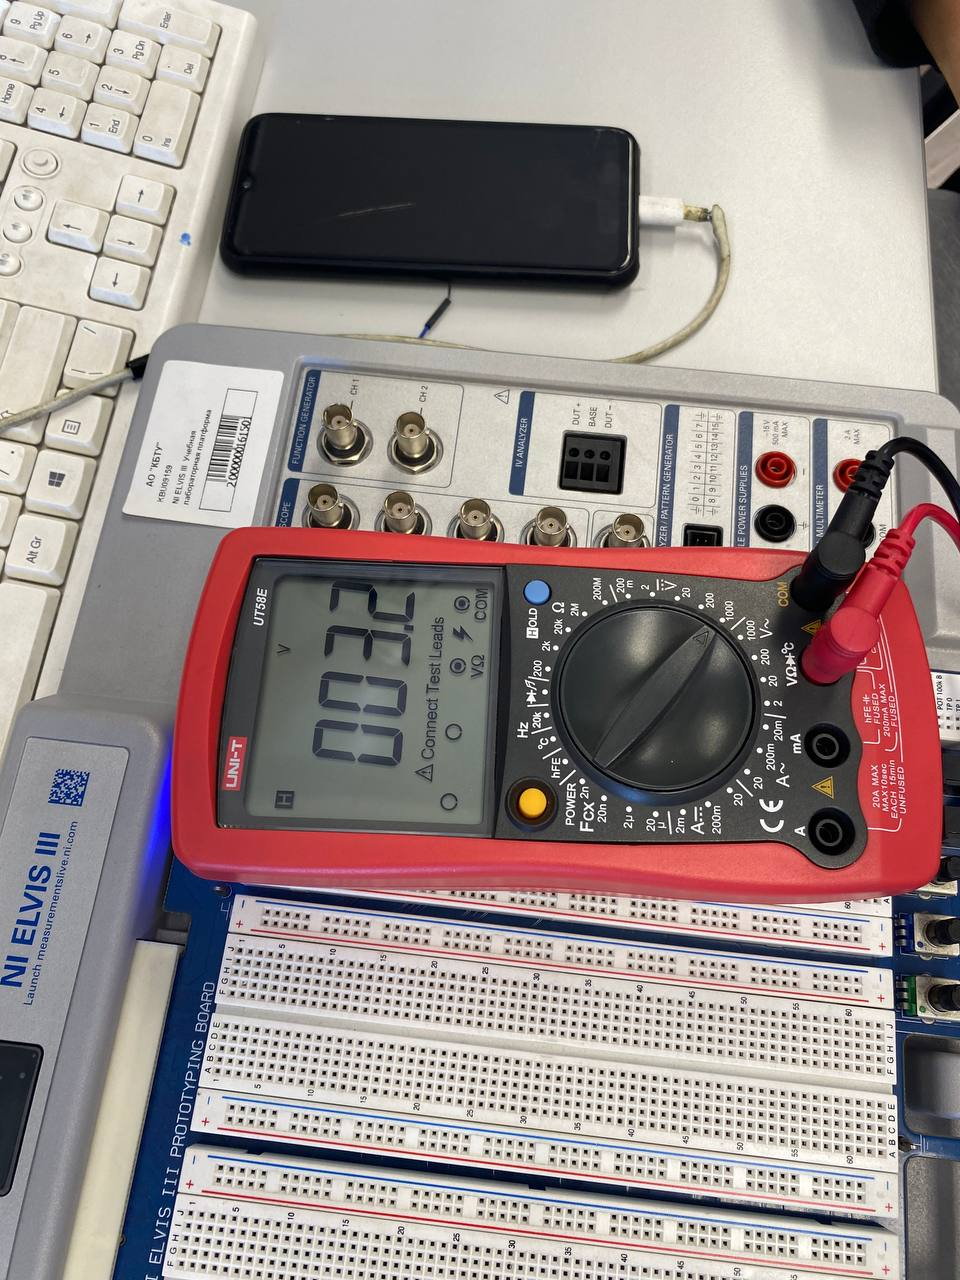
\includegraphics[width=14cm]{images/photo1696868902.jpeg}
\end{flushleft}

\begin{flushleft}
    \begin{titlepage}
    \centering
    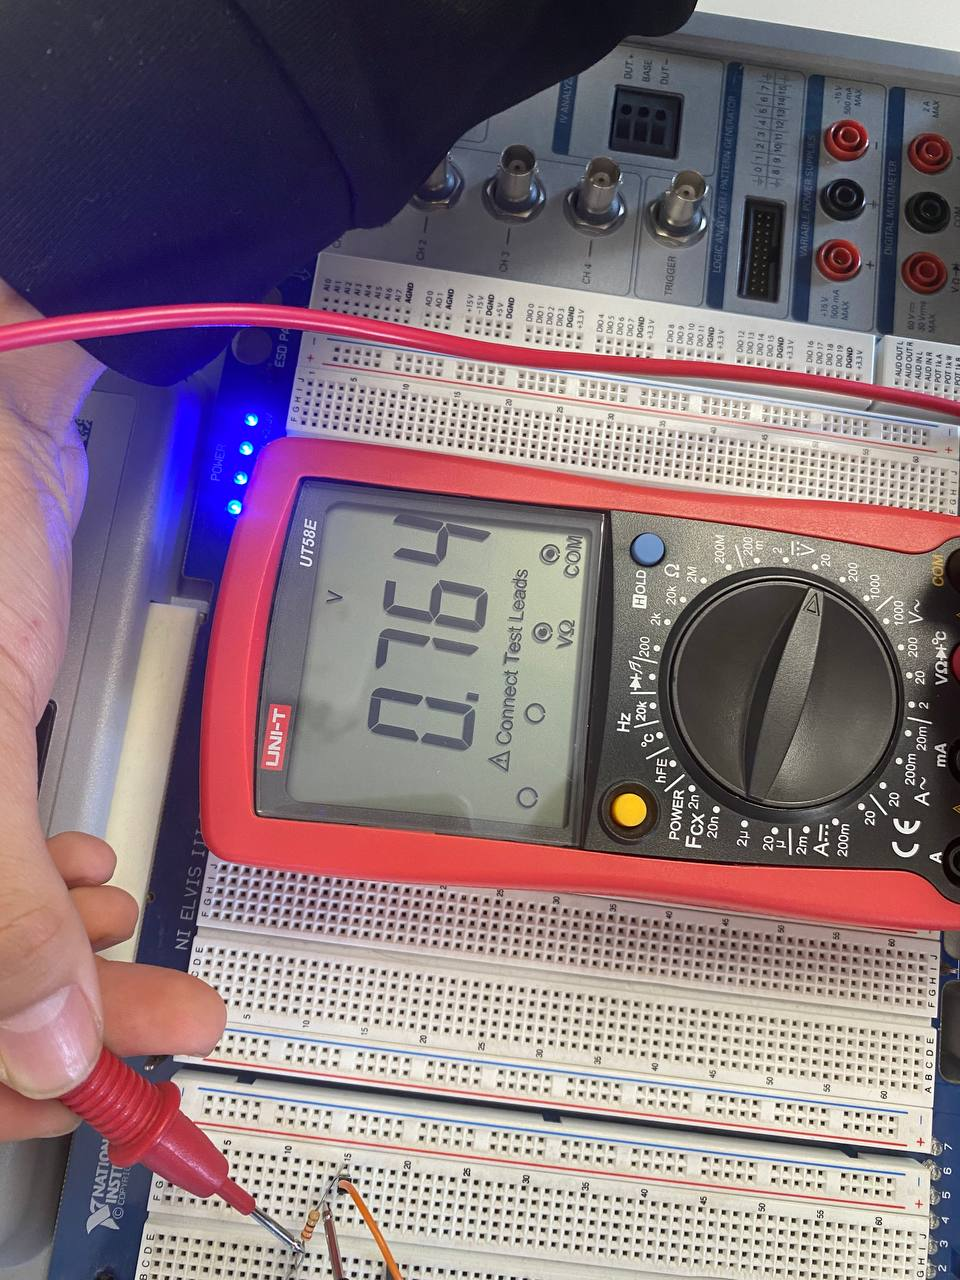
\includegraphics[width=14cm]{images/photo1696237774.jpeg}
\end{flushleft}

\begin{flushleft}
    \begin{titlepage}
    \centering
    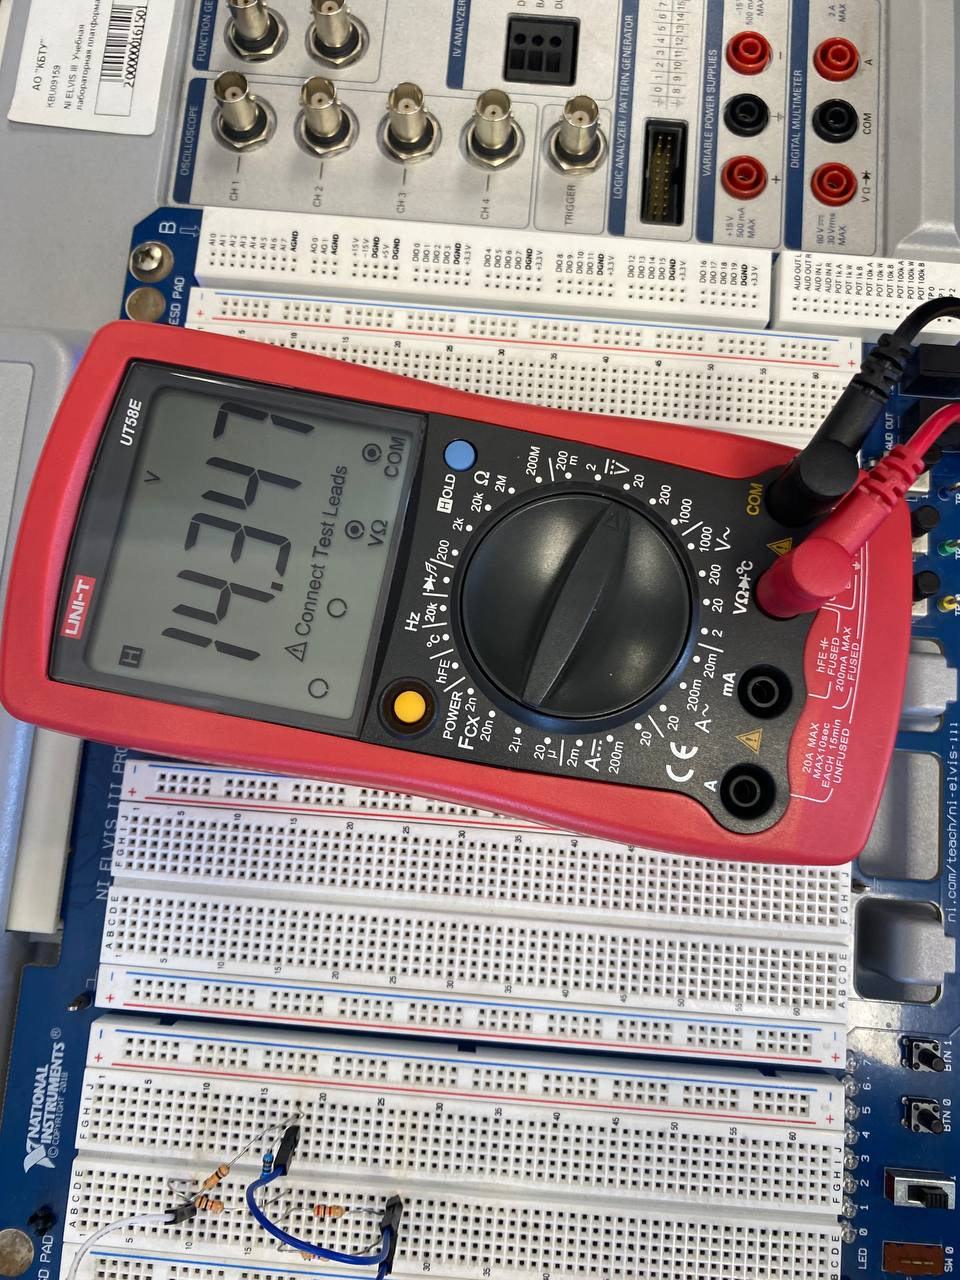
\includegraphics[width=14cm]{images/photo1696868902 (3).jpeg}
\end{flushleft}


\begin{flushleft}
    \begin{titlepage}
    \centering
    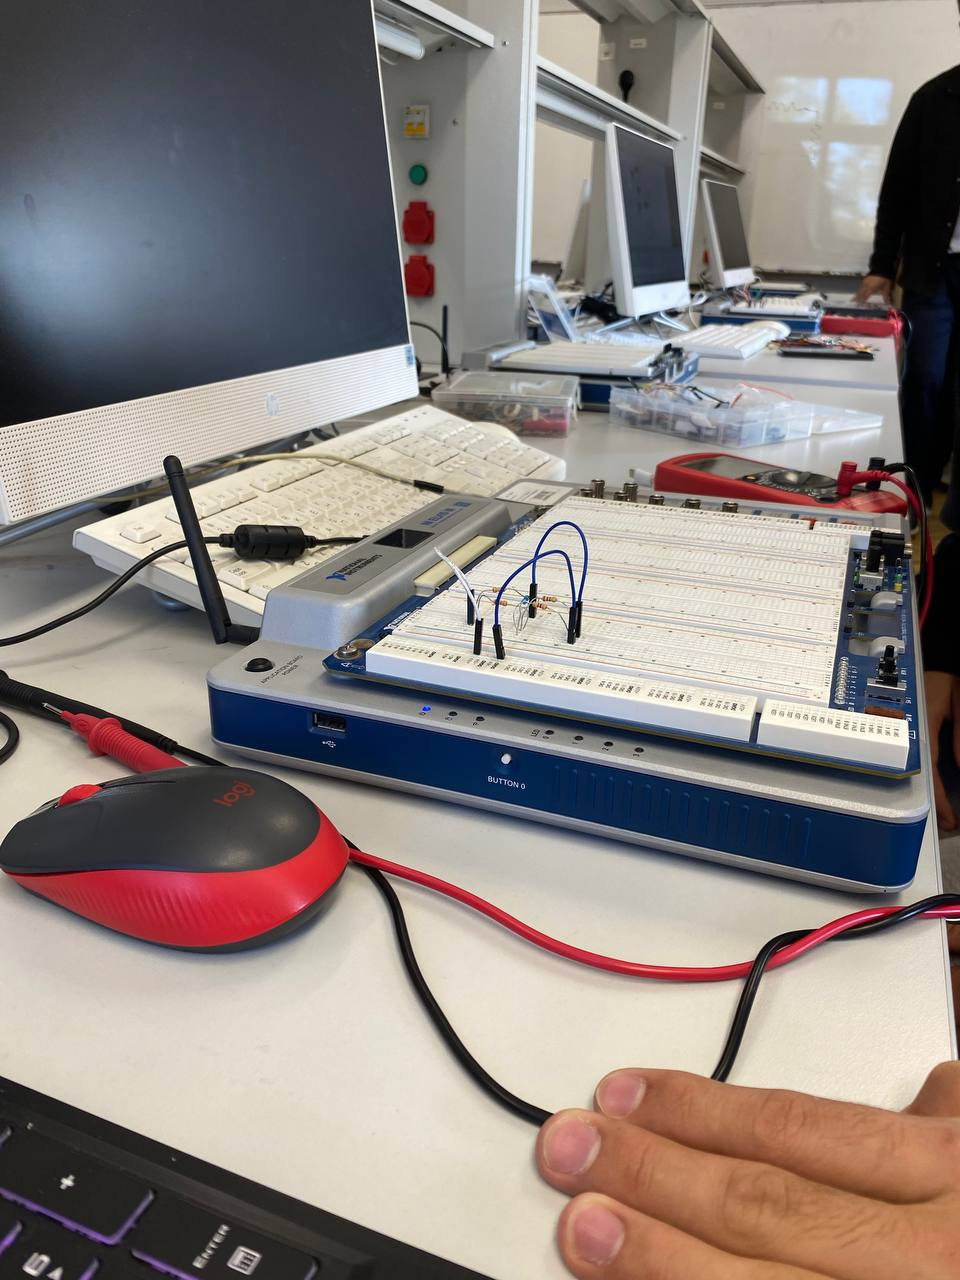
\includegraphics[width=15cm]{images/photo1696868715.jpeg}
\end{flushleft}


\begin{flushleft}
\textbf{Conclusion:}
The laboratory session provided a profound exploration into the various techniques employed in electrical circuit analysis. By delving into methods ranging from Kirchhoff's laws, which form the foundational principles of circuit behavior, to more intricate techniques like Mesh and Nodal analyses, we equipped ourselves with tools essential for dissecting and understanding intricate circuits.
 \end{flushleft}
\end{document} 
